
To provide an overview of all the topics that will be addressed, we will begin by defining the key components of this thesis and explaining the basics to build upon in the later chapters. 

\section{Web Applications}
\label{sec:webapp}
A \textit{web application} has been defined as “a software application, executed by a web server, which responds to dynamic web page requests over HTTP” by the Web Application Security Consortium WASC~\cite{noauthor_web_2012}. 
In simpler terms, a web application is software that runs on a server and users access it through a web browser (like Chrome or Firefox) over the internet.

Typically, the resources and scripts of web applications — such as images, text, or functionalities — are requested by the client, which is the user's computer or device, using a web browser or similar tools. This interaction follows a set of rules known as the Application Programming Interface (API), which specifies what requests can be made and how the server should respond.
The~\autoref{fig:simplified-web-app} illustrates the basic communication process between the client (the user's device), the server (where the application runs), and external services (such as another server).

Most web applications also use a database, which is a structured way of storing data, to keep information consistently available and reliable. For the purposes of this thesis, we assume that the web application is written fully in JavaScript, and has a monolithic architecture. This means that it operates as a single cohesive program on a physical computer, rather than being divided into separate parts that run on different cloud services (like AWS, or Amazon Web Services, which offers online computing power without needing dedicated hardware\footnote{https://aws.amazon.com/})
Additionally, we assume the server follows Representational State Transfer (REST) principles, which are common API design practices to enable smooth communication as described by \citet{roy_t_fielding_rest_2008}. 

The web server processes requests that adhere to the Hypertext Transfer Protocol (HTTP) standard, which is the foundational protocol used for transmitting data on the web (ref. ~\autoref{tab:rest_http_methods}). It can be used  with the database operations, commonly known as CRUD (acronym for Create, Read, Update and Delete)  operations, as established by \citet{martin_managing_1983}, when a web application utilizes a persistent database.
This adherence ensures that the server and client can operate independently, meaning they can be developed and updated separately without affecting each other\cite{fielding_http_2022}.



\begin{figure}[t]
    \centering
    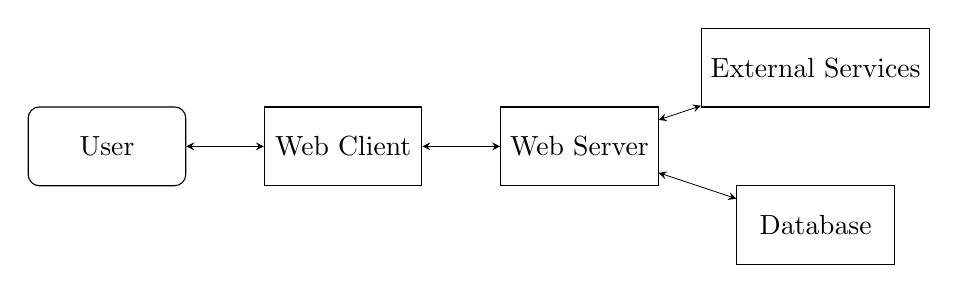
\begin{tikzpicture}[node distance=3cm]
    % Define styles for nodes and arrows
    \tikzstyle{user} = [rectangle, rounded corners, minimum width=2cm, minimum height=1cm, text centered, draw=black]
    \tikzstyle{browser} = [rectangle, minimum width=2cm, minimum height=1cm, text centered, draw=black]
    \tikzstyle{server} = [rectangle, minimum width=2cm, minimum height=1cm, text centered, draw=black]
    \tikzstyle{database} = [rectangle, minimum width=2cm, minimum height=1cm, text centered, draw=black]
    \tikzstyle{external} = [rectangle, minimum width=2cm, minimum height=1cm, text centered, draw=black]
    % Use arrows with both directions
    \tikzstyle{arrow} = [thick, <->, >=stealth]
% Arrow style for double lines

    \tikzset{doubleArrow/.style={thick, <->, >=stealth,
        line width=0.1mm, line cap=round, draw=black
    }}
    % Nodes
    \node (user) [user] {User};
    \node (browser) [browser, right of=user] {Web Client};
    \node (server) [server, right of=browser] {Web Server};
    \node (database) [database, right of=server, yshift=-1cm] {Database};
    \node (external) [external, right of=server, yshift=1cm] {External Services};
    % Arrows (connections)
    \draw  [doubleArrow](user) -- (browser);
    \draw  [doubleArrow](browser) -- (server);
    \draw  [doubleArrow](server) -- (database);
    \draw [doubleArrow] (server) -- (external);
    \end{tikzpicture}
    \caption{Structure of a simplified Web Application}
    \label{fig:simplified-web-app}

\end{figure}

\begin{table}[t]
    \centering
    \begin{tabular}{@{}lll@{}}
        \toprule
        \textbf{HTTP Method} & \textbf{Purpose}                         & \textbf{Idempotent} \\ \midrule
        GET                   & Retrieve a resource                     & Yes                 \\
        POST                  & Create a new resource                   & No                  \\
        PUT                   & Update or create a resource             & Yes                 \\
        PATCH                 & Partially update a resource             & Yes (mostly)        \\
        HEAD                  & Retrieve headers of a resource         & Yes                 \\
        OPTIONS               & Return available HTTP methods           & Yes                 \\
        DELETE                & Remove a resource                       & Yes                 \\ \bottomrule
    \end{tabular}
    \caption[List of HTTP Methods]{Summary of REST HTTP Methods and their idempotence \cite[chapter 9]{fielding_http_2022}}
    \label{tab:rest_http_methods}
\end{table}

\section{Cross-Site Scripting}
\label{sec:xss}
\textit{Cross-site scripting} (XSS) is a security vulnerability that enables the execution of malicious code on a remote server or
another client by exploiting weaknesses in server-side input validation. \cite{bisht_xss-guard_2008}
According to the Open Web Application Security Project (OWASP) top 10 list, XSS, and other code injection techniques, are the second most common vulnerabilities in web applications, only surpassed by broken access control.\cite{noauthor_owasp_2025}

\citet{kieyzun_automatic_2009} describe two kinds of XSS attacks: reflected, or non-persistent, XSS and persistent XSS.
\subsection{Reflected XSS}
A \textit{reflected} XSS vulnerability occurs when an application incorporates part of the user’s input into the HTML page it generates without proper validation or encoding. Attackers often leverage social engineering tactics to persuade victims to click on a disguised URL that includes malicious HTML or JavaScript code. When the user's browser processes this URL, it renders the HTML and executes the embedded JavaScript, potentially leading to the theft of sensitive information such as cookies and other user data.

To mitigate the risk of reflected XSS attacks, users should be vigilant about checking link anchors before clicking on them, ensuring they recognize the source of the URL. Additionally, applications can protect against such vulnerabilities by rejecting or sanitizing input values that might contain script code, thereby preventing malicious content from being observed or executed in a browser context.

\subsection{Persistent XSS}
A \textit{persistent} XSS vulnerability arises when an application saves an attacker's input in a database. Later, this malicious content is retrieved and included in HTML pages that are served to multiple users, such as in a chat application.

Preventing persistent XSS is generally more complex than addressing reflected XSS, as developers need to ensure that input values are adequately sanitized or rejected not only during user submission but also when the data is retrieved for HTML rendering. This requires implementing various sanitization techniques for inputs that may contain SQL code used in database commands, as these can also create security vulnerabilities. An SQL injection is always possible, when a server uses the naive method of string concatenation.

The query \lstinline{q = "INSERT INTO Students VALUES ('" + FName.Text } 
\lstinline{+ "', '" +LName.Text} \lstinline{ + "')";} is an example for this naive query generation, as any input for FName.Text and LName.Text is taken verbatim, which opens the query database injections. If a malicious attacker used \lstinline{Robert'); DROP TABLE STUDENTS; --) } for FName.Text, the query would execute two statements: \lstinline{INSERT INTO Student Values ('Robert');} and \lstinline{DROP TABLE STUDENTS;}. First, these queries insert the value into the database, and then delete the table. 

Persistent XSS, therefore, can have a more severe impact than reflected XSS for two main reasons. First, it removes the necessity for social engineering tactics; attackers can directly insert malicious scripts into the system without needing to deceive users into clicking on a link. Second, a single malicious script stored in the database can run on the browsers of many users, significantly amplifying the potential damage done by the attack.


\autoref{fig:xss-simp} illustrates a simplified scenario in which persistent XSS can be employed to execute code on another machine by sending malicious code to the server, which subsequently transfers this malicious code to unsuspecting clients. A common instance of this vulnerability occurs when an application provides a web interface that allows users to enter and store text without adequate server-side input validation and sanitization, thereby failing to prevent users from executing inserted scripts on the devices of other users.

A recent example of this would be a vulnerability in the web interface web UI of Cisco Enterprise Chat and 
Email\footnote{https://www.cisco.com/c/en/us/support/docs/csa/cisco-sa-ece-xss-CSQxgxfM.html, last accessed on 4/4/2025}. 
Cisco is a company that develops communication and security-related tools, 
underscoring the critical need for rigorous testing for vulnerabilities,
as even organizations specializing in security can overlook certain issues.

The severity of a vulnerability hinges on the accessibility of the exploit. 
If an attack requires authentication and allows for traceability,
it may represent a minor inconvenience and therefore calls for a patch of the issue,
as the attacker can be identified. However, if an XSS attack can be executed anonymously,
this poses a significant risk to all users and requires immediate remediation.


%\clearpage
\begin{figure}[t]
\centering
\begin{adjustbox}{height=7cm}
\begin{tikzpicture}[node distance=1cm]

\tikzstyle{startstop} = [rectangle, rounded corners, minimum width=3cm, minimum height=1cm,text centered, draw=black, fill=red!30]

\tikzstyle{process} = [rectangle, minimum width=3cm, minimum height=1cm,text centered, draw=black, fill=orange!30]
\tikzstyle{decision} = [diamond, minimum width=3cm, minimum height=1cm, text centered, draw=black, fill=lmugreen!69]
\tikzstyle{arrow} = [thick,->,>=stealth]



\node (start) [startstop] {Malicious Attacker Client};
\node (pro1) [process, below = of start] {\lstinline{ <script>alert("Hello")</script>}};
\node (dec1) [decision, below = of pro1] {Server};
\node (pro2a) [startstop, below  = of dec1, xshift=-3cm] {Unassuming Client};
\node (pro2b) [startstop, below  = of dec1, xshift=3cm] {Unassuming Client};
\node (stopA) [process, below = of pro2a] {Hello};
\node (stopB) [process, below = of pro2b] {Hello};


\draw  [arrow](start) -- node[anchor=east] {post message} (pro1);
\draw  [arrow](pro1) -- node[anchor=east] {store message}(dec1);
\draw  [arrow](dec1) -- node[anchor=east] {distribute message} (pro2a);
\draw [arrow] (dec1) -- node[anchor=west] {distribute message} (pro2b);
\draw [arrow] (pro2a) -- node[anchor=west] {execute code}(stopA);
\draw [arrow] (pro2b) -- node[anchor=west] {execute code}(stopB);
\end{tikzpicture}
\end{adjustbox}      
    \caption[Simplified XSS attack example]{An example of a persistent XSS attack. A malicious attacker sends a message to the server that contains a script, which will be distributed to clients. Upon receiving the message, the script will be executed.}
    \label{fig:xss-simp}
\end{figure}

\newpage
\section{Testing}
The next aspect we would like to concentrate on is the testing of a web application. First we define what “testing” means, then look into the methodology of “fuzzing” as a technique used to test.

At its essence, \textit{testing} constitutes the systematic process of validating and verifying the functionality of a program. A sensible analogy for the concepts of validation and verification was articulated by \citet{b_w_boehm_verifying_1984}:

\begin{itemize}[label={}]
    \item \textit{Verification}: “Am I building the product right?” 
    \item \textit{Validation}: “Am I building the right product?”
\end{itemize}



Depending on the nature of the testing methodology employed, different levels of  assessment can be achieved. A unit test, which is designed to evaluate a single component or function—hence the term “unit”—primarily provides insights into the correctness of that individual function. \cite{beck_test-driven_2003}

In contrast, an end-to-end test, while potentially less precise in verifying the functionality of individual components, serves to validate the overall functionality of the entire system, with all components integrated. \cite{paul_end--end_2001}

Another dimension of testing relates to the approach to how a program can be analysed.
\textit{Static} analysis involves examining the source code or structure of a program without executing it. This technique is typically applied during the development process and can identify potential errors, coding standard violations, and security vulnerabilities by analysing the program's syntax and control flow. However, one limitation of static analysis is the potential for false positives, where the tool flags code as problematic even when it functions correctly. 
\textit{Dynamic} analysis, in contrast, examines a program while it is running, assessing its behaviour in real time. This technique allows for observation of the program's execution. By monitoring the program during execution, dynamic analysis can identify issues such as memory leaks and runtime errors that may not be apparent through static analysis. However, dynamic analysis requires the program to be executed, which can limit testing in situations where running the software is impractical or impossible. \cite{hennell_comparison_1990}\cite{umar_comparative_2021} 

Independently of the type of testing and the methodology employed, a program can accommodate a vast array of potential inputs. Manually identifying all possible variations can be impractical, as the number of combinations can quickly become overwhelming. To address this challenge, we can utilize a technique known as “fuzzing”. 


\section{Fuzzing}
\label{sec:fuzzing}
\textit{Fuzzing} is an automated process that involves the generation of input data to identify potential program errors, commonly referred to as “bugs”, which may arise from unhandled cases. These cases can include scenarios such as incompatible data types, excessively large entities, or the presence of unexpected characters.
The most basic idea of fuzzing is generating random input strings, which already found bugs and crashes in the tested libraries on first use.~\cite{miller_empirical_1990}\\
Fuzzing can be done in different ways, and in the following we will describe the two most commonly used types: “white-box” fuzzing and “black-box” fuzzing.
Internally, the generation of inputs can be done by either generating new inputs every time, or by mutating an existing input and using this as a new baseline.~\cite{van_sprundel_fuzzing_2005}

\vspace{0.5cm}
\begin{tabular*}{\textwidth}{@{}c|c@{}}[t]
    
\begin{minipage}{\dimexpr0.5\textwidth-2\tabcolsep}
\centering
    % Left Diagram - White Box Fuzzing
    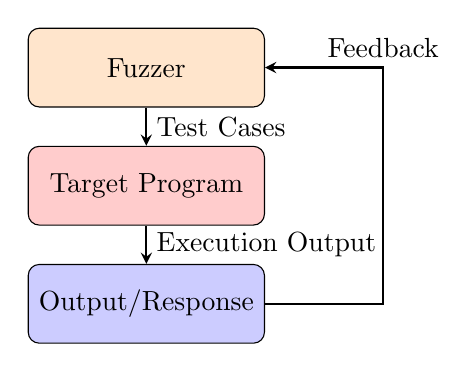
\begin{tikzpicture}[node distance=1.5cm]
                % Define styles for nodes and arrows
        \tikzstyle{box} = [rectangle, rounded corners, minimum width=3cm, minimum height=1cm, text centered, draw=black, fill=blue!20]
        \tikzstyle{fuzzer} = [rectangle, rounded corners, minimum width=3cm, minimum height=1cm, text centered, draw=black, fill=orange!20]
        \tikzstyle{target} = [rectangle, rounded corners, minimum width=3cm, minimum height=1cm, text centered, draw=black, fill=red!20]
        \tikzstyle{arrow} = [thick,->, >=stealth]
        \tikzstyle{title} = [rectangle, rounded corners, minimum width=5cm, text centered, draw=none, fill=none, font=\large\bfseries] 
    
        \node (fuzzer) [fuzzer] {Fuzzer};
        \node (target) [target, below of = fuzzer] {Target Program};
        \node (output) [box, below of = target] {Output/Response};

        % Arrows
        \draw  [arrow](fuzzer) -- (target) node[midway, right] {Test Cases};
        \draw [arrow] (target) -- (output) node[midway,right] {Execution Output};
        \draw [arrow] (output.east) --+(1.5,0) |- (fuzzer.east) node[midway, above] {Feedback};
    \end{tikzpicture}

\end{minipage}
&
\begin{minipage}{\dimexpr0.5\textwidth-2\tabcolsep}
\centering

    % Left Diagram - White Box Fuzzing
    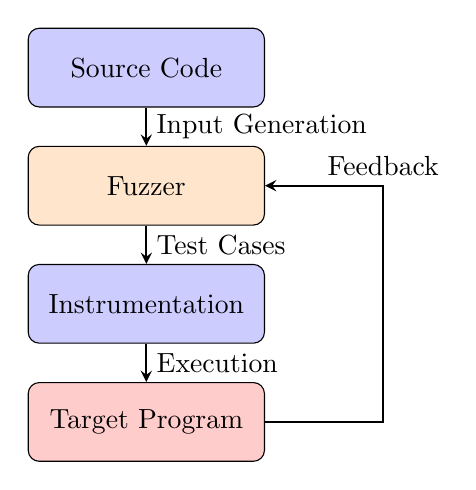
\begin{tikzpicture}[node distance=1.5cm]

        \tikzstyle{box} = [rectangle, rounded corners, minimum width=3cm, minimum height=1cm, text centered, draw=black, fill=blue!20]
        \tikzstyle{fuzzer} = [rectangle, rounded corners, minimum width=3cm, minimum height=1cm, text centered, draw=black, fill=orange!20]
        \tikzstyle{target} = [rectangle, rounded corners, minimum width=3cm, minimum height=1cm, text centered, draw=black, fill=red!20]
        \tikzstyle{arrow} = [thick,->, >=stealth]
        \tikzstyle{title} = [rectangle, rounded corners, minimum width=5cm, text centered, draw=none, fill=none, font=\large\bfseries]
        \node (source) [box] {Source Code};
        \node (fuzzer) [fuzzer, below of = source] {Fuzzer};
        \node (instr) [box, below of = fuzzer] {Instrumentation};
        \node (target) [target, below of = instr] {Target Program};

        % Arrows
        \draw  [arrow](source) -- (fuzzer) node[midway, right] {Input Generation};
        \draw  [arrow](fuzzer) -- (instr) node[midway, right] {Test Cases};
        \draw  [arrow](instr) -- (target) node[midway, right] {Execution};
        \draw  [arrow](target.east) -- +(1.5,0) |- (fuzzer.east) node[midway, above] {Feedback};

    \end{tikzpicture}
    
\end{minipage}

\\

\begin{minipage}[t]{\dimexpr0.5\textwidth-1\tabcolsep}
\captionof{figure}{Simplified black-box fuzzing process}
    \label{fig:black-box-testing}

\end{minipage}
&
\begin{minipage}[t]{\dimexpr0.5\textwidth-1 \tabcolsep}
\captionof{figure}{Simplified white-box \\fuzzing process}
\label{fig:white-box-testing}

\end{minipage}

\end{tabular*}

\subsection{Black Box Fuzzing}
\label{sec:black-box}

The fuzzer created by \citet{miller_empirical_1990} is an example of what was later defined as \textit{black-box fuzzing}.

The key characteristic of black-box fuzzing is its lack of insight into the internal design and logic of the software being tested.  
The fuzzer generates inputs that it feeds to the target program and based on the feedback and result of these inputs it can discover unhandled exceptions, missing input validation or unintended behaviour.~\cite{godefroid_fuzzing_2020}
A simplified test flow can be seen in \autoref{fig:black-box-testing}.
Black-box fuzzing is always a dynamic analysis, as the program under test has to be running.




\subsection{White Box Fuzzing}
\label{sec:white-box}
Since the black-box fuzzer has no insights into the source code or specifications, it discovers branches of the execution by chance.

\textit{White box fuzzing} is a technique that tries to alleviate this chance by gathering insights about the system under test by instrumenting the code and shadowing the execution, as depicted in \autoref{fig:white-box-testing}.
The term white-box fuzzing was coined by \citet{godefroid_automated_2008} and first implemented in their symbolic execution engine \textbf{SAGE} \cite{godefroid_sage_2012}. Symbolic execution is the underlaying process of exploring a program.
A common example of the power of white-box fuzzing, and therefore symbolic execution,  is a simple conditional such as \lstinline+if(x == 5) then+. While in black-box fuzzing the chance to meet this condition is 2\textsuperscript{64} if x is a random 64-bit value, a white-box fuzzer could note the condition \lstinline+x==5+ and generate both inputs that satisfy and don't satisfy this condition, no longer reliant on chance. \cite{godefroid_automated_2008}

While black-box fuzzing is always a dynamic analysis as the program has to be executed, white-box fuzzing could be used for both dynamic and static analysis, as it has access to the code and even combined approaches are possible \cite{artho_combined_2005}.



\section{Dynamic Symbolic Execution}
\label{sec:dse}
\textit{Dynamic symbolic execution} (DSE), a concept first presented in the seventies \cite{boyer_selectformal_1975}\cite{king_new_1975}\cite{king_symbolic_1976}, and is regarded as a form of white-box fuzzing that merges concrete execution with symbolic reasoning. This integration transforms it into a dynamic code analysis technique, as the system under test is actively executed. The aforementioned SAGE engine is one notable implementation that employs this concept.

In DSE, each variable holds both a symbolic value and a concrete value, making the approach commonly referred to as “concolic execution”. This term reflects the combination of symbolic and concrete values, highlighting how DSE allows for the effective exploration of executable paths while accommodating both concrete inputs and symbolic reasoning. 

The \textit{symbolic} part of the variables holds the variable state and the conjunction of encountered conditionals, e.g. \lstinline[language=JavaScript]+if (x === 0)+, called a \textit{path condition}. 
It enables the engine to create \textit{concrete} inputs that match the path condition of the symbolic variable and its negation. 
The conditional
\lstinline[language=JavaScript]+if (x === 0)+ would therefore lead to the inputs 
\lstinline[language=JavaScript]+x = 0+ and
\lstinline[language=JavaScript]+x = 1+ with 1 being an arbitrarily chosen value. The symbolic variable also holds the state of the variable, i.e. the transformations applied to it, such as 
\lstinline[language=JavaScript]@x = x + 1@, 
which adds the state
$X \rightarrow X+1$
 with 
$X$ being the initial input.




We can denote the state of the concolic variable $x$ as a tuple of $(pc, S(x), C(x))$


\capstartfalse
{\centering
    \begin{table}[ht]
        \begin{tabular}{lll}
            where & pc & the path condition \\
             & $S(x) \rightarrow X$& \specialcell[c]{the symbolic state of X,\\ i.e. the applied transformations on the initial value}\\
             & $C(x) \rightarrow 0$& the concrete value of x\\
        \end{tabular}
    \end{table}
\par} 
\capstarttrue

DSE can be grouped into online and offline execution strategies. 
In the context of \textit{online} DSE, both symbolic and concrete execution occurs in real time as the program operates. 
The execution mechanism explores program paths dynamically, solving constraints on-the-fly whenever branches are encountered. 
This method offers immediate feedback and allows for improved coverage of execution paths since it can adapt to the dynamic conditions inherent in the program environment. 
However, online execution may also experience performance overhead due to the simultaneous management of both execution and constraint solving. 
On the other hand, \textit{offline} execution focuses on the static analysis of a program’s code without executing it in real-time. 
Rather than exploring paths dynamically, offline DSE generates a manageable set of test inputs for later execution. 
This methodology is advantageous as it can leverage complete path exploration techniques that are unconstrained by the immediacy of execution. 
Moreover, offline methods can be more efficient for producing a wide array of test cases. 
However, they often lack the capacity to adapt to dynamic environmental changes, potentially overlooking vulnerabilities that manifest only under specific runtime conditions. \cite{andreasen_survey_2018}


Prominent tools that leverage DSE methodology include \textbf{KLEE}
\cite{cadar_klee_2008}, \textbf{DART} \cite{godefroid_dart_2005}, and \textbf{EXE} \cite{cadar_exe_2008},
and for this thesis we use the DSE engine \textbf{ExpoSE} \cite{loring_expose_2017} for JavaScript. 

KLEE is an online symbolic execution engine recognized for its ability to automatically generate high-coverage tests for complex programs. It efficiently explores numerous execution paths while detecting bugs through its symbolic execution capabilities, allowing it to handle real-world programs of considerable complexity while minimizing the performance overhead commonly associated with conventional execution methods. 

DART (Directed Automated Random Testing) merges random testing with online dynamic analysis with the goal of automated united testing.

Similarly, EXE employs DSE techniques for the automatic detection of security vulnerabilities in executable programs, which allow it to explore execution paths by solving path constraints effectively during runtime.

In this thesis, we use the DSE engine ExpoSE, which has a strong focus on string manipulations and generating inputs based on regular expressions. 




\subsection{Example Dynamic Symbolic Execution}
In this subsection, we will demonstrate the concept of DSE by employing the code in \autoref{lst:example-program}. 
To facilitate the process, we can first depict the program as a Control Flow Graph (CFG) as seen in \autoref{fig:example-program-graph}. 
The CFG displays the conditions and transformations along its edges, with the vertices signifying the state of the program.
On entering  the program, we assume that the initial value is x=1 and y=0, just to tell the DSE Engine the types of the variables, and to give it a starting point. 


\begin{tabular*}{\textwidth}{@{}c|c@{}}
\begin{minipage}{\dimexpr0.5\textwidth-2\tabcolsep}
\centering
\begin{lstlisting}[language=JavaScript]
    function g(x, y) {
        if (x !== y){
            x += y
        }
        else {
            if (y > 8){
                y+=1
            }
        }
        x += 1
        if (x !== 0 )
        { 
          if ( y != 0){
            x = y
          }
        }
    }
\end{lstlisting}
   
\end{minipage}
&
\begin{minipage}{\dimexpr0.5\textwidth-2\tabcolsep}
\centering
     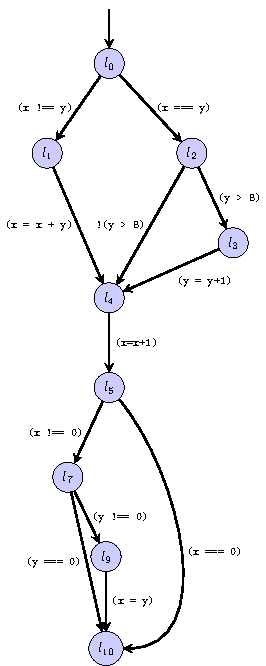
\includegraphics{../luatex/cfg/out/cfg.pdf}
\end{minipage}
\\

\begin{minipage}[t]{\dimexpr0.5\textwidth-1\tabcolsep}
 \captionof{lstlisting}{A simple program}
\label{lst:example-program}

\end{minipage}
&
\begin{minipage}[t]{\dimexpr0.5\textwidth-1 \tabcolsep}
\captionof{figure}{CFG of \autoref{lst:example-program}}
\label{fig:example-program-graph}

\end{minipage}

\end{tabular*}


In similar fashion, we can now walk through the execution, and create a branch whenever we encounter diverging paths.
For example, right at the start, we have two possible routes the execution can take: $x == y$ and $\neg(x == y)$.
We can now construct the symbolic execution tree displayed in \autoref{fig:symbolic-execution-tree} by tracking the path conditions and transformations of the variables.

\begin{sidewaysfigure}[t]
  \centering
  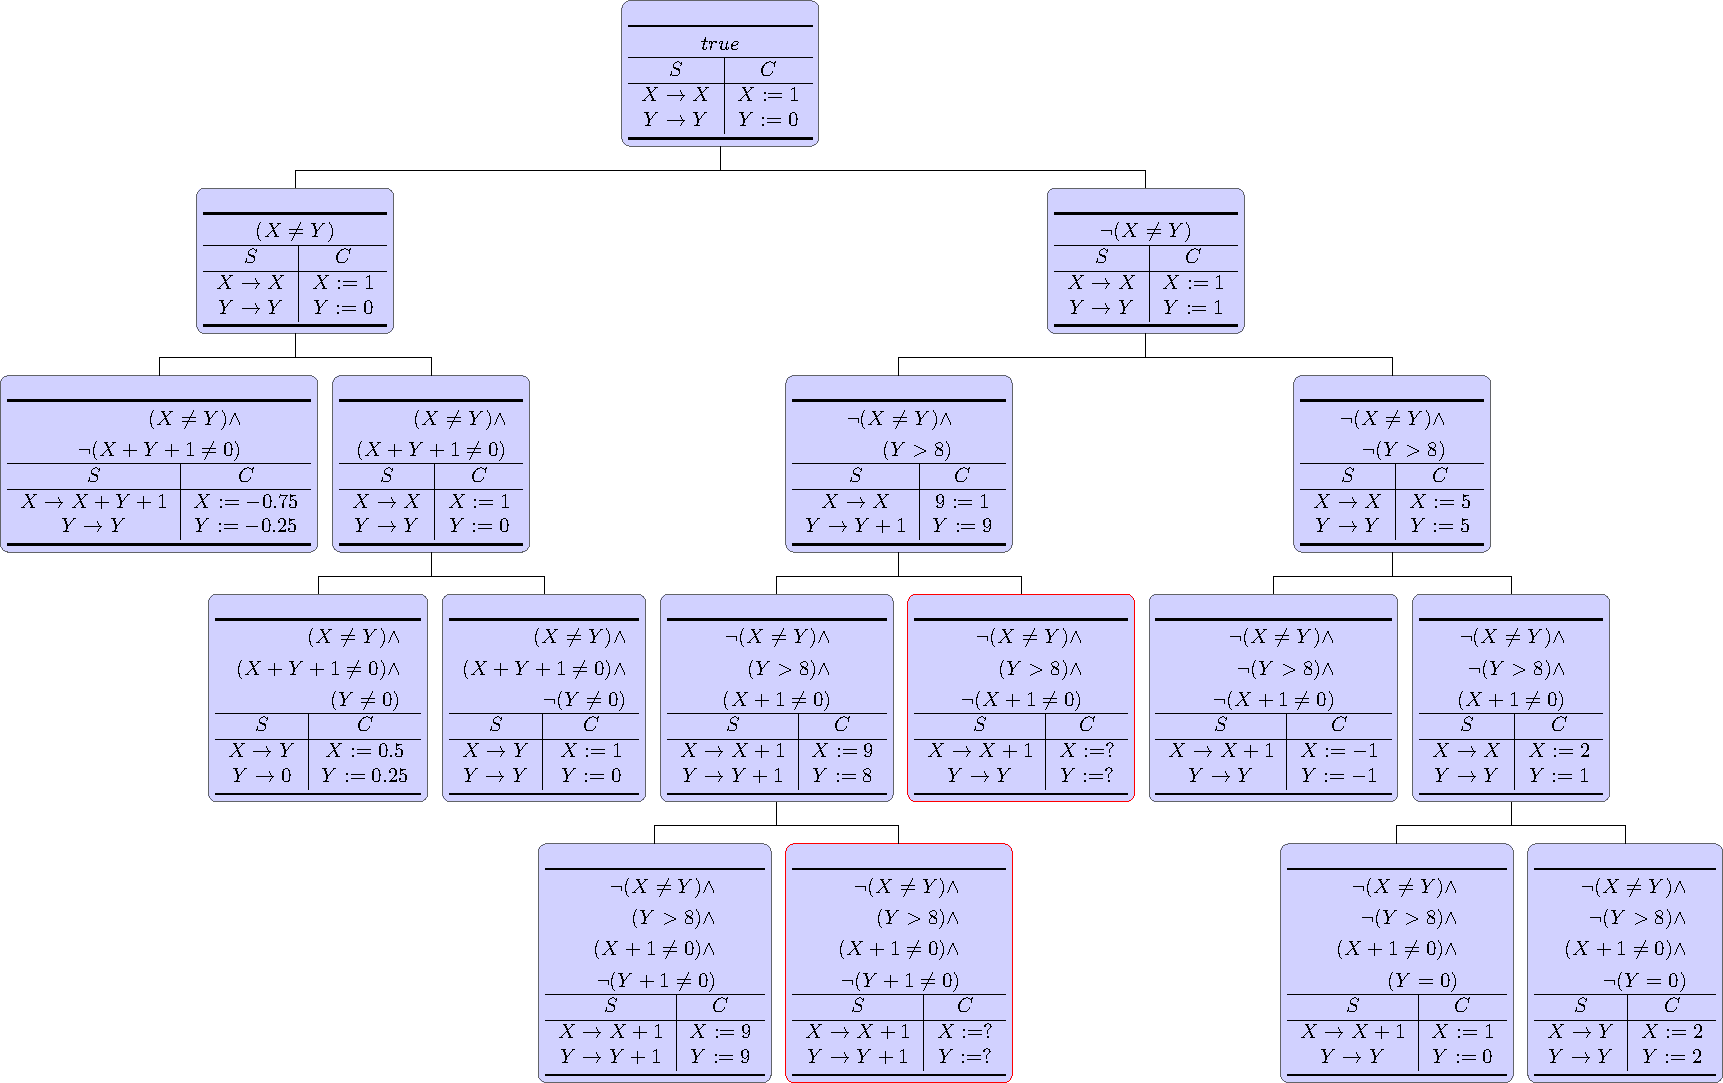
\includegraphics[width=\textwidth]{../luatex/symexe/out/symexe.pdf}    
  \caption[Symbolic execution tree]{Symbolic execution tree of \autoref{lst:example-program}, displaying the path condition and the concolic state. Unreachable paths are highlighted in red.}
  \label{fig:symbolic-execution-tree}
\end{sidewaysfigure}




After constructing the execution tree, we can generate distinct inputs for each of the leaf nodes, checking for satisfiability.
For instance, if we want to determine which input would cover the branch in the middle of the tree, we can do so by solving the constraints  $(\neg(X \neq Y) \land (Y > 8) \land \neg( X+1==0 ) \land \neg(Y+1 \neq 0 ))$. 
Solving these constraints yields the answer of (x = 9, y = 9), which indicates that this input will satisfy the specified conditions for that branch. 
Any condition that cannot be satisfied means that the leaf node cannot be reached, no matter the input. The two leafs highlighted in red in  \autoref{fig:symbolic-execution-tree} showcase this.
These constraints are usually solved by a Satisfiable Modulo Theories (SMT) Solver, which we will briefly explain in \autoref{sec:z3}.


JavaScript has a few peculiarities, as it is dynamically typed and therefore only resolved at runtime. 

\subsection{Limitations DSE}

As with any explorative system, DSE has limitations regarding its capabilities. 
The most significant limitation is computable paths, which have the potential to explode if the analysed program is not designed with DSE in mind, for instance, if it heavily relies on recursive calls. 
But even with DSE in mind, the paths grow exponentially with the number of conditionals in a program.  \cite{cadar_symbolic_2013}
This also occurs with symbolic addresses, as it has to account for any possible memory address a variable can occupy.\cite{elkarablieh_precise_2009}  

To address this, most DSE frameworks employ various kinds of techniques for reducing the number of paths. 
One such technique is path merging based on heuristics, where a reoccurring conditional, can be merged into one (for example in a loop).\cite{kuznetsov_efficient_2012}

\citet{cha_unleashing_2012} propose a solution for a symbolic memory, reducing the possible paths for symbolic addresses by concretizing writes and only allowing symbolic reads.    

It also is not suitable for full boundary testing, as DSE checks for reachability, and once a path is covered, it will not move back and check for edge cases in this path, possibly missing unexpected behaviour, i.e. catching an integer overflow.\cite{berthier_efficient_2023}




